\documentclass[12pt,a4paper]{article}
\usepackage[T1]{fontenc}
\usepackage[utf8]{inputenc}
\usepackage[margin=25mm]{geometry}
\usepackage{graphicx,booktabs,amsmath,array,microtype,xcolor}
\usepackage[labelfont=bf,font=small]{caption}
\usepackage[hidelinks]{hyperref}
\usepackage{float,fancyhdr}
\setlength{\parindent}{0pt}
\setlength{\parskip}{5pt plus 1pt}
\fancyhf{}\fancyfoot[C]{\thepage}\renewcommand{\headrulewidth}{0pt}\pagestyle{fancy}
\newcommand{\panel}[3]{\begin{minipage}[t]{#1}\centering\includegraphics[width=\linewidth]{#2}\\[2pt]{\small #3}\end{minipage}}
\begin{document}
\begin{center}
{\Large\bfseries Pool-ball localisation and recognition}\\[3pt]
Manon Yiqin Galian Ng (23375206) --- CSU44053
\end{center}

% CHANGE: OVerall this is pretty good as a base. BUT this doesn't really sound like a third year computer science student

% CHANGE: when you add figure could you also add a comment saying where you took the image or data (csv) from

% CHANGE: i also want to tell a good story

\section{Processing and design}
% CHANGE: this can said simpler

The system locates balls and assigns type, colour and identity. AllBalls supplies
parameter selection and colour references; Tables1--6 supply repeatedly inspected
validation images rather than an independent test set.

\begin{figure}[H]\centering
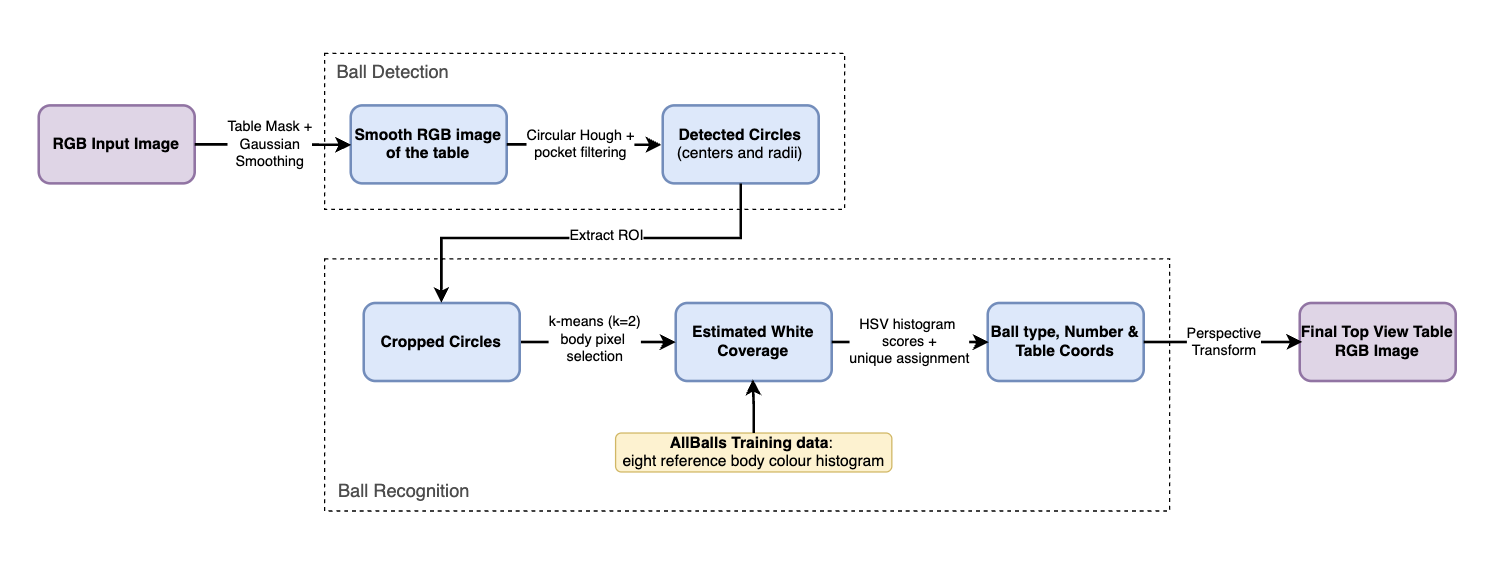
\includegraphics[width=\linewidth]{assets/pipeline.png}
\caption{Final Detection and Recognition pipeline.}
\end{figure}
\subsection{Table restriction and circular detection}
% CHANGE: multiple things to change here:
% 1. its called the circula hough transform
% 2. if this is not standard:$5\times5$ Gaussian, $\sigma=1.5$ then we need to explain why
% 3. the first sentence doesn't make much sense so maybe we want to reword and also explain why

The quadrilateral through $(337,35)$, $(1570,21)$, $(1888,451)$ and $(38,472)$ masks
the background. Greyscale intensities are smoothed with a $5\times5$ Gaussian,
$\sigma=1.5$. Circular Hough voting [1] estimates centres and radii before perspective
correction, which could distort ball outlines.

% CHANGE: multiple things to change here:
% 1. we need to explain why we wanted to do this grid search (beause manual selection was difficult to understand which config to put)
% 2. the selected setting could be worded better
% 3. we should also explain the rational behind pocket filtering and its limitation
A 480-configuration search on AllBalls ranked matched balls first, then fewer false
detections and lower centre error. Selected settings: accumulator resolution ratio
1.5, centre separation 18 pixels, edge threshold 75, centre-vote threshold 35, and
radii 15--30 pixels. Candidates within 25 table units of six approximate pocket
centres are rejected; this is an exclusion threshold, not a measured pocket radius.

% CHANGE: we probably want an image od the detected circles (maybe we can omit the the table mask image and have the detedtec balls on the masked image)
\begin{figure}[H]\centering
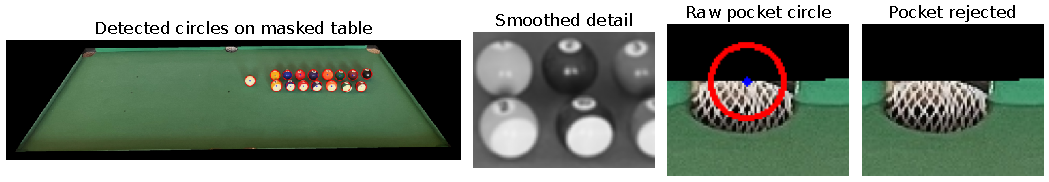
\includegraphics[width=.90\linewidth]{assets/detection_stages.pdf}
\caption{AllBalls: full table mask, smoothed ball detail, and the same pocket
before/after filtering. The raw 17 candidates become 16 matched detections.}
\end{figure}
\newpage

\subsection{Ball regions, type estimation and colour references}
% CHANGE: multiple things to change here:
% 1. we should explain why extracted the ball crops
% 2. we can word this more simply
% 3. what does thsi even mean? Only masked pixels enter recognition; the crop is clipped at the image boundary.
% 4. also we are getting the colour clusters with K means but never mentioning it
% 5. this also doesn't means anything: Spatial position is not a clustering feature: disconnected patches may share a cluster.
%       but we can use it as an into to the fact that we did try CCA later to see if spacia positioning would improve stuff
Each retained circle defines a square colour crop and a circular pixel mask.
Only masked pixels enter recognition; the crop is clipped at the image boundary.
Two BGR clusters estimate the proportions of light and non-light material. The
fixed clustering seed and three initialisations make the comparison reproducible;
termination uses at most 50 iterations or a centre-change threshold of 0.2.
Spatial position is not a clustering feature: disconnected patches may share a cluster.

% CHANGE: multiple things to change here:
% 1. we also need to explain how we chose these params and thresholds (i belive we did a grid searxh actually right? maybe we need to add that to the final repot)
% if we did not do a grid search than we have to explain that they were chosen manually by exmamining the pictures and then the perforamce we good on allballs so no need to do a grid search
A cluster's representative colour is converted to HSV. It is light when
$V\ge170$ and $S\le165$; otherwise $V\le90$ denotes dark material. Cluster
proportions estimate the light fraction $w$. The initial classification is cue-like
white for $w\ge0.85$, solid for non-light coverage at least 70\%, and striped for
other mixtures with both light and non-light material. These manually selected
rules estimate visible appearance, not the ball's hidden surface.

% CHANGE: definitly to save we can make these smaller and the caption and be simplier
\begin{figure}[H]\centering
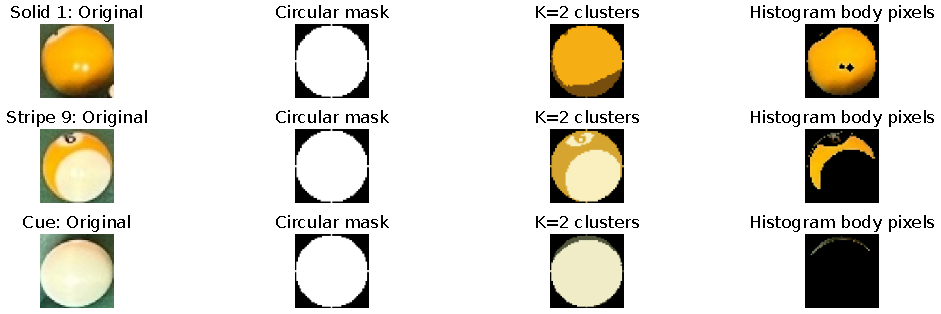
\includegraphics[width=\linewidth]{assets/recognition_stages.pdf}
\caption{Original crops, extraction masks, two-cluster segmentation and selected
histogram pixels. Rows show yellow solid 1, yellow stripe 9 and a cue. Black
outside the masks means excluded pixels. The cue is not a body-colour reference.}
\end{figure}

% CHANGE:
% 1. this can be written much better
% 2. explain the rational behind this also: $3\times3$ elliptical erosion
% 3. also need to explain this: bright, low-saturation pixels are excluded using the light thresholds above
% 4. also we need to explain why we decieded to add the histogram reference (remeber we are telling a story!)
Eight HSV reference histograms describe yellow, blue, red, purple, orange, green,
maroon and black. AllBalls detections are matched to its labelled centres to obtain
reference identities and crop radii; the 15 numbered balls supply the examples.
Solid/striped partners contribute to the same colour model. The cue is excluded.
A $3\times3$ elliptical erosion reduces crop-edge contamination; bright,
low-saturation pixels are excluded using the light thresholds above. Fewer than
12 retained pixels means no numbered-colour evidence.

% CHANGE:
% 1. we need to explain this a bit: $18\times8\times8=1152$
% 2. again same this can be written better
% 3. this needs to be explained also: A separable $[1,2,1]/4$ filter
Histograms have $18\times8\times8=1152$ bins over hue $[0,180)$ and saturation/value
$[0,256)$. Near-neutral pixels with BGR channel range below 15 receive hue zero,
reducing instability in almost grey colours. A separable $[1,2,1]/4$ filter smooths
bins, wrapping hue and clamping the other endpoints. Each descriptor sums to one;
normalised reference examples are pooled and normalised again. This represents
colour distributions rather than a single dominant hue, at the cost of discarding
spatial arrangement. The settings are a practical compromise, not demonstrated optima.

\newpage

\subsection{Soft evidence and joint identity assignment}
% CHANGE: 
% 1. agin we need to explain why we shifted to soft scores
% 2. does the formula come from my lecture notes
% 3. we need to explain the scores a lot more
For normalised query histogram $p$ and reference $q_c$, body-colour similarity is
one minus Bhattacharyya distance:
\[
s_c=1-\sqrt{1-\sum_b\sqrt{p_bq_{c,b}}}.
\]
These eight similarities are not probabilities and need not sum to one. Colour
alone cannot distinguish solid/striped partners, which share a reference.

% CHANGE:  
% 1. we need to explain all these formulas
% 2. maybe also need to explain the graphs (how did you generate these?)
The final recogniser retains type uncertainty. Preferred light-fraction intervals
$I_t$ are solid $[0,0.30]$, stripe $[0.30,0.85]$ and cue $[0.85,1]$. With distance
$d$ to an interval (zero inside), compatibility and identity scores are
\[
g_t(w)=\exp\!\left[-\frac{d(w,I_t)^2}{2(0.10)^2}\right],\quad
S_n=s_{c(n)}g_{t(n)}(w),\quad S_0=w g_{\rm cue}(w).
\]
Support decreases smoothly outside each interval; width 0.10 controls tolerance.

\begin{figure}[H]\centering
\panel{.47\linewidth}{assets/type_support.pdf}{Soft type support}\hfill
\panel{.51\linewidth}{assets/colour_scores.pdf}{Measured Table2 similarities}
\caption{Yellow partners have similar colour preferences but different white coverage.}
\end{figure}

% CHANGE:  
% 1. we need to explain why we decided to do this
% 2. also need to explain that we used the hungrain method and why
Maximum-weight one-to-one assignment enforces each identity at most once [2].
Separate dummy choices allow multiple Unknowns. Unusable evidence or scores at most
$10^{-9}$ are ineligible. This is not calibrated rejection: weak extra candidates
can still take real identities.

% CHANGE:  
% 1. we prob need to explain a lot more why we did these cue specific tunings (and show images of the the smaller white circle)
% 2. should also explain that instead of using the larger radius heuristic (which works in this case but might not generalise well) we could have built a system to get the expected diameter of the balls at each depth since they would all have the smae diameter
% 3. also for the heuristic the reason behind it is that even with the depth, in genreal the size different would still work
Initially white ROIs are expanded by one radius pixel and reanalysed, without
changing stored detection geometry. When multiple original candidates are white,
the largest original Hough radius reserves cue identity. The original classifications
determine this selection even if expansion changes the evidence.

% CHANGE:  
% 1. for the white path image maybe don't use the green stiped ball because it looks too simiarl
% 2. also make the image smaller
\begin{figure}[H]\centering
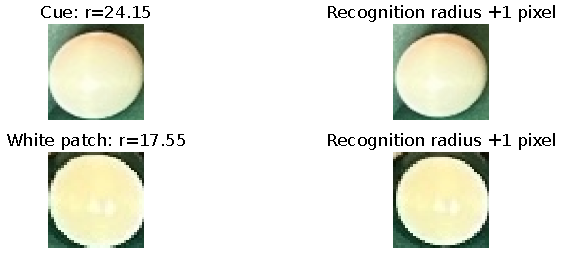
\includegraphics[width=.55\linewidth]{assets/white_padding.pdf}
\caption{Table1 cue and white patch before/after expansion. The patch's light
coverage falls from 100\% to 93.98\%, but it remains Unknown: padding is not a general repair.}
\end{figure}
\newpage
\subsection{Table coordinates and final representation}

% CHANGE:  
% 1. i don't think this wording is neceaary: homography maps
% 2. do we need this formula? can't we just say we used perspective shift? 
A homography maps the supplied corners to $(0,0)$, $(1433,0)$, $(1433,682)$ and
$(0,682)$ in a $1434\times683$ rectangle:
\[
\lambda(x_t,y_t,1)^T=H(x,y,1)^T.
\]

% CHANGE: 
% the wording can be simpler here. 
% how did we get thsi value: Diagram balls have nominal 43\,mm diameter
% all of this mkaes no sense, and why are we even saying it? identity, not observed orientation. Because visible ball centres lie above the cloth, the cloth-plane homography can introduce systematic position error.
Extraction uses original-image circles; transformed centres supply evaluation and
overhead positions. At the supplied scale, table units are approximately millimetres.
Diagram balls have nominal 43\,mm diameter; their bands depict identity, not observed
orientation. Because visible ball centres lie above the cloth, the cloth-plane
homography can introduce systematic position error.

% CHANGE: 
% Let's use the AllBalls image references
\begin{figure}[H]\centering
\panel{.32\linewidth}{../final_output/final/Table2/original_numbered.png}{Original labels}\hfill
\panel{.32\linewidth}{../final_output/final/Table2/table_numbered.png}{Rectified labels}\hfill
\panel{.32\linewidth}{../final_output/final/Table2/table_diagram.png}{Identity diagram}
\caption{Table2: all genuine identities are correct; an extra detection remains Unknown.}
\end{figure}


\subsection{Alternatives Considered}

% CHANGE: 
% all of this doesn't explain why we wanted to do it or how we selected the params. Or why we didn't choose better params
% we should add images for CCa also
\textbf{Spatial type information.} CCA measures light/non-light component counts,
largest areas and light coverage in an inner boundary band. Eight-connected components
smaller than 2\% of ROI area are ignored in component statistics. A $5\times5$ erosion
defines the band. Fixed rules test whether spatial features distinguish stripe whites
from highlights/number patches, using identical detections and K=2 segmentations.
The stripe rule needs a light component covering at least 20\% of the ROI,
light on at least 20\% of the boundary band, and at least 10\% non-light area.

% CHANGE:
% same as above
\textbf{Additional detections.} Nearby baseline circles are grouped using disks
expanded to 1.4 times their radii. Groups with at least two detections receive local
Hough searches with vote threshold 22 and centre separation 12 pixels. Cloth rejection uses HSV
$35\le H\le95$, $S\ge35$, $V\ge30$, a $9\times9$ table inset and $3\times3$
closing. Duplicate/pocket proposals are removed;
baseline circles remain.

% CHANGE:
% same as above
Optional watershed uses candidate centres as markers and non-foreground as background.
Additional circles need basin-supported foreground area 0.15--2.0 times their disk
area. Watershed filters proposals; it does not invent centres.

% CHANGE:
% it is not clear why we chose these images
\begin{figure}[H]\centering
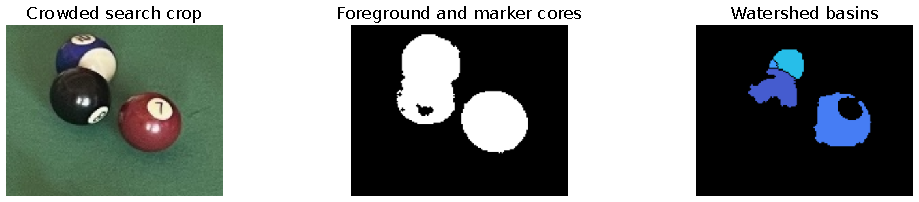
\includegraphics[width=.88\linewidth]{assets/guided_stages.pdf}
\caption{An actual Table3 search region, foreground with marker cores, and watershed
basins. Coloured regions are segmentation labels, not ball identities.}
\end{figure}

\newpage
\section{Results and analysis}
\subsection{Evaluation protocol and final performance}

% CHANGE:
% do we need the formulas? maybe the localisation one but the others?
Tables1--6 contain 90 annotated balls. Detected centres are matched one-to-one to
annotations within 15 rectified table units. Matching maximises valid pairs; proximity
orders alternatives but does not guarantee globally minimum total distance. A matched
circle is a true positive (TP), an unmatched circle a false positive (FP), and an
unmatched annotation a false negative (FN). Pooled counts give

\[
P=\frac{TP}{TP+FP},\quad R=\frac{TP}{TP+FN},\quad
F_1=\frac{2TP}{2TP+FP+FN},\quad
\bar e=\frac{1}{TP}\sum_i\|\hat{\mathbf x}_i-\mathbf x_i\|_2.
\]

% CHANGE: we can explain this better
For $C$ correctly numbered matched balls, identity accuracy is $C/TP$ and
end-to-end correct-identity recall is $C/N$, where $N$ is the annotation count.
Misses and Unknowns on genuine balls reduce the latter; surplus detections are
penalised by detection precision, not directly by $C/N$. Colour evaluation excludes
the six cues. AllBalls is excluded from pooled validation results because it supplies
reference colours and detection tuning. The annotation file is BallLocations.csv.

% CHANGE: can we make this shorter in length
\begin{table}[H]\centering
\caption{Final pipeline on every validation image. Centre error is in table units;
identity fractions use matched detections.}
\begin{tabular}{lrrrrrr}\toprule
Image & GT & TP & FP & FN & Mean error & Correct IDs\\\midrule
Table1 &16&14&1&2&7.68&11/14\\
Table2 &16&16&1&0&3.58&16/16\\
Table3 &16&15&0&1&3.12&15/15\\
Table4 &15&14&0&1&3.89&14/14\\
Table5 &14&14&0&0&5.83&13/14\\
Table6 &13&13&0&0&5.76&11/13\\\midrule
Pooled &90&86&2&4&4.91&80/86\\\bottomrule
\end{tabular}
\end{table}

% CHANGE: we can explain this better: The pooled localisation error weights each image by its matched detections, rather than averaging image means equally
Detection precision is \textbf{97.73\%}, recall \textbf{95.56\%} and F1
\textbf{96.63\%}. Final identity accuracy is \textbf{93.02\%} on matched balls;
end-to-end recall is \textbf{88.89\%}. The pooled localisation error weights each
image by its matched detections, rather than averaging image means equally.

\begin{table}[H]\centering
\caption{Standalone appearance estimates versus final joint recognition.}
\begin{tabular}{lrr}\toprule
Stage & Correct / matched & Correct / annotated\\\midrule
Initial type &76/86 (88.37\%)&76/90 (84.44\%)\\
Body colour, excluding cue &73/80 (91.25\%)&73/84 (86.90\%)\\
Final identity &80/86 (93.02\%)&80/90 (88.89\%)\\\bottomrule
\end{tabular}
\end{table}

% CHANGE: this can be explained simpler
These measure different stages: final identities also use soft compatibility,
white-crop expansion and global uniqueness. Their gains cannot be attributed to
any individual addition without an isolated ablation. The six cues are all correct;
AllBalls also gives 16/16 identities, but that is reference-image performance.

\newpage
\subsection{Scene-level successes and failures}

% CHANGE: caption can be simpler
\begin{figure}[H]\centering
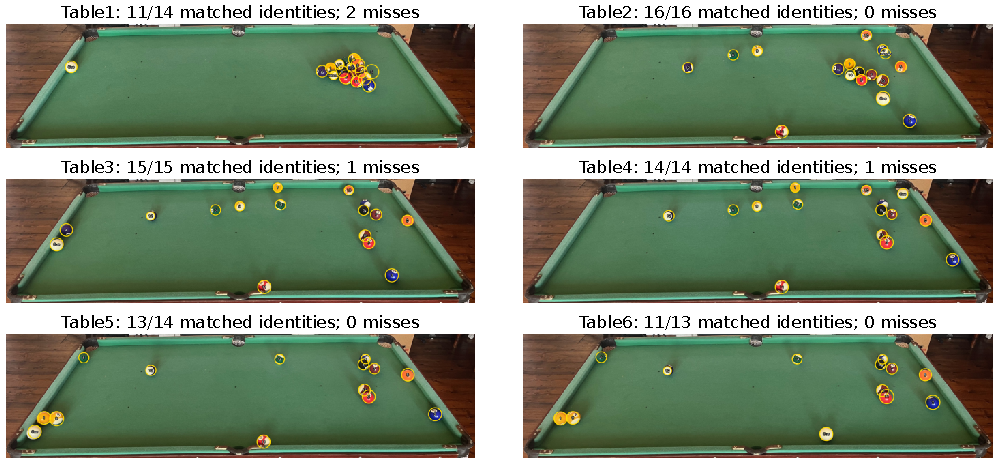
\includegraphics[width=.94\linewidth]{assets/final_gallery.pdf}
\caption{All six validation outputs. Fractions count correct matched identities;
they are not complete-scene accuracy. False detections and Unknowns remain visible.}
\end{figure}

% CHANGE: what does this paragraph add? 
Table2 identifies every genuine ball but retains a false circle as Unknown.
Tables3 and 4 identify every match but miss blue stripe 10. Tables5 and 6 miss no
balls yet make identity errors: detection and recognition fail separately.

% CHANGE: 
% what does this paragraph add?
% what does this mean: Displaced crops can corrupt recognition even when centres count as detected. 
Table1 misses balls 6 and 7, leaves stripe 14 Unknown, exchanges identities 5 and 9,
and labels a false circle 6. The exchanged matches have centre errors 14.63 and
14.81, near the 15-unit tolerance. Displaced crops can corrupt recognition even
when centres count as detected.

% CHANGE
% the analyse of our system can be much better

% CHANGE
% not sure what these pictures are means to say? be definitly need some but why these ones? maybe there are better ones
\begin{figure}[H]\centering
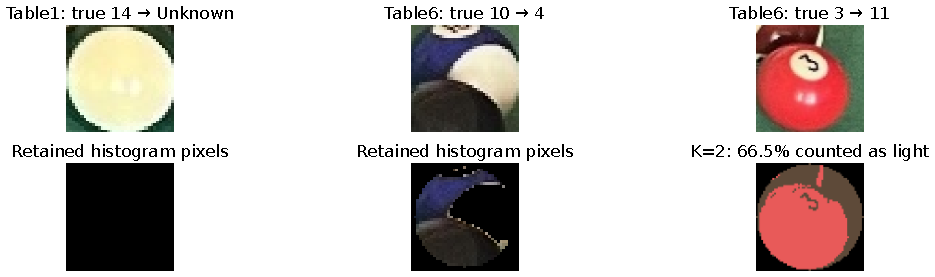
\includegraphics[width=.90\linewidth]{assets/failure_details.pdf}
\caption{Table1 white patch; Table6 blue stripe 10 assigned 4; Table6 red solid 3
assigned 11. Titles give matched truth; image labels are predictions.}

\end{figure}

% CHANGE: this is not well written at all. I understand what you are trying to say but as is it makes no sense
In Table6, red solid 3 has strongest red similarity but 66.53\% estimated light
coverage, favouring stripe 11. Blue stripe 10 scores 0.52 against black, 0.43 purple
and 0.24 blue. Final identity 4 reflects ambiguous colour \emph{and} unique-assignment
competition, not simply the best histogram match. Visible stripe area, illumination
and crop displacement are plausible contributors, not isolated causal findings.
The Table1 patch still lacks usable body-colour evidence after expansion.
\newpage

% CHANGE: in general maybe for the experiments we should explain then and also evaluate them together this would make
% the paragraph a bit shorte becyse we don't have to repear stuff. Also it makes more sense to add the eperiments after our resulst
% because these are experiments we did to try to upgrade our system but didn't include them for X or Y reason.
% also we should also show that the reason we didn't include them is not becaues they are bad but because either
% the simpler version was perform approx the same or better and thus we couldn't justify the added complexity
% one goal of the project is also to build a system that could also be generatlise to other pool ball games (given the same angle of the table)
% OR if you think it makes more sense the experiment section would be befor ethe limitations part of the report or before the final eval
\subsection{What the controlled experiments show}

% CHANGE: explain simpler bu tthis paragra is not too bad actually
\textbf{K=2 with CCA.} On 86 matched balls, correct types fall from 76 to 73:
zero corrections and three regressions. Two cues become striped (Tables2 and 3), as
does a solid in Table4. Light-region size and boundary coverage satisfy the tested
stripe rule despite these identities. Connectivity is not a unique stripe signature.

\begin{figure}[H]\centering
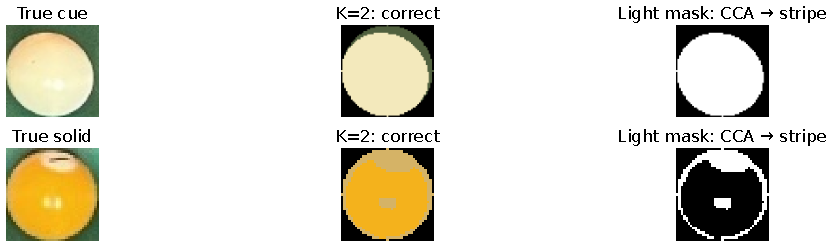
\includegraphics[width=.74\linewidth]{assets/cca_examples.pdf}
\caption{CCA regressions: Table2 cue and Table4 solid, both initially correct.
Their light masks trigger the fixed stripe rule.}
\end{figure}
\textbf{Guided detection and unchanged recognition.} All variants use identical
reference histograms, recognition settings and unique assignment.
\begin{table}[H]\centering
\caption{Pooled results. NFP: false detections assigned real identities.
Correct identities are out of 90 annotations.}
\begin{tabular}{lrrrrrr}\toprule
Detection &TP&FP&FN&F1 (\%)&Correct IDs&NFP\\\midrule
Baseline &86&2&4&96.63&80&1\\
Guided Hough &89&8&1&95.19&81&6\\
Guided + watershed &88&6&2&95.65&80&5\\\bottomrule
\end{tabular}
\end{table}
% CHANGE: explain simpler bu tthis paragra is not too bad actually
Guided Hough recovers three misses, raising recall to 98.89\%, but adds six false
detections and only one net correct identity. Watershed removes two false positives
and one recovered ball, leaving no identity gain. On Table3, an extra candidate
takes identity 12 from a previously correct ball: assignment cannot absorb all extras.
\begin{figure}[H]\centering
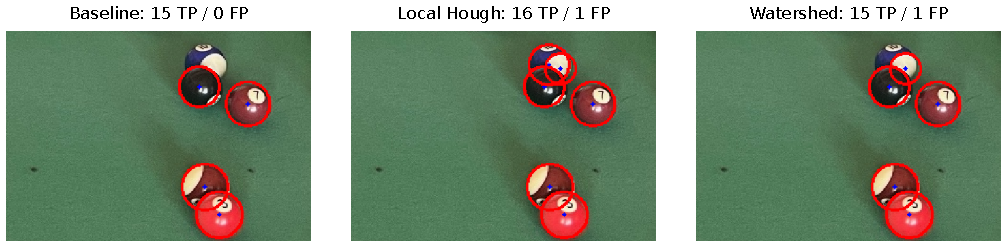
\includegraphics[width=.94\linewidth]{assets/guided_details.pdf}
\caption{The same Table3 window: local Hough recovers a ball with a false circle;
the watershed area check rejects the recovery but retains that false circle.}
\end{figure}

% CHANGE: explain simpler 
% also use the feedback I gave above for the experiments to make this better
The baseline was retained for fewer false numbered outputs and lower complexity.
Guided Hough remains promising for recall. These results concern the tested settings;
different segmentation, markers, features or tuning could change either experiment.
\newpage
\subsection{Group performance, robustness and improvements}

% CHANGE: I think I like this grpah but I am not 100% what the y axis is its not very clear and the groups also are not super clear
\begin{figure}[H]\centering
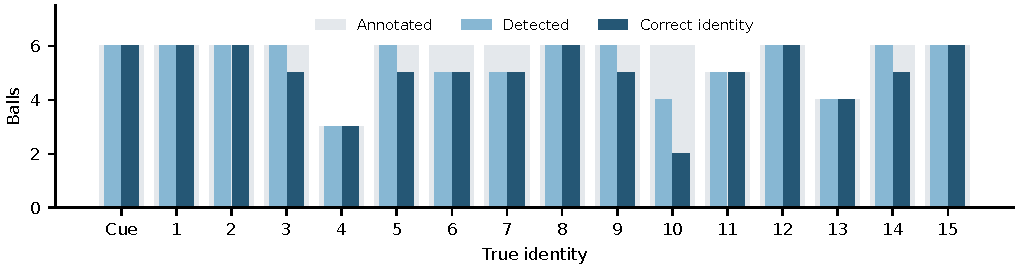
\includegraphics[width=.94\linewidth]{assets/identity_counts.pdf}
\caption{Counts by true identity: annotated examples, matched detections and correct
final identities. Unequal sample counts remain visible.}
\end{figure}

% CHANGE: we should try to find an explanation for these strengths and weakness based on the system we desiged
Blue stripe 10 is weakest: six annotations yield four detections and two correct
identities (33.3\% end-to-end). Solids give 41/45 correct (91.1\%), stripes 33/39
(84.6\%) and cues 6/6. Some perfect identities have only three or four examples;
these identify development weaknesses, not reliable generalisation rates.

% CHANGE: this can be shortened and explained a lot better
\textbf{Appropriateness and scene changes.} Circular voting suits visible outlines,
histograms summarise colour variation, and uniqueness uses a physical constraint.
However, radius limits, supplied corners and pocket locations depend on the camera.
New resolution/viewpoint requires updated geometry and size ranges. A nearer white
patch can exceed a distant cue's radius. Lighting and camera response change both
histograms and white coverage; occlusion removes circle and stripe evidence.

% CHANGE: this can be shortened and explained a lot better
\textbf{Limits of validation.} Repeated inspection of six images from one scene
introduces selection bias. One recovered identity changes end-to-end recall by
1.11 percentage points, insufficient to establish robustness. Freeze settings before
testing new photographs with varied lighting, viewpoint, orientation and crowding.
The 15-unit tolerance is about 35\% of nominal ball diameter; evaluate sensitivity
to stricter tolerances rather than adjusting it to raise scores. Centre annotations
cannot establish segmentation or boundary accuracy.

% CHANGE: this can be explained a lot better
\textbf{Targeted improvements.} More varied labelled references and illumination
normalisation could improve colour stability. Adaptive table geometry and size priors
could support new cameras. A validated Unknown policy could prevent weak proposals
taking identities. Improve foreground/marker construction while tracking corrections
\emph{and} regressions: green-cloth rejection can remove green balls, and crowded
windows cannot recover isolated misses. Assess detection and final identities together;
attractive segmentation alone is not evidence of improved performance.

\paragraph{References and assistance}
[1] K. Dawson-Howe, CSU44053 Computer Vision course material, Trinity College Dublin.\par
[2] H. W. Kuhn, ``The Hungarian method for the assignment problem,''
\emph{Naval Research Logistics Quarterly}, 2, 83--97 (1955).\par
ChatGPT/Codex assisted with programming, diagnostics and report drafting. Results
and illustrations come from application outputs and recorded report diagnostics.
\end{document}
